%        File: 03140299_kentaro_wada.tex
%     Created: Tue Jul 21 02:00 AM 2015 J
% Last Change: Tue Jul 21 02:00 AM 2015 J
%
\documentclass[10pt,twocolumn]{jarticle}

%%% Packages ----------------------------------------
% to input Japanese
\usepackage[japanese]{babel}

%% something
% \usepackage{ascmac}

% to be standard a4paper
\usepackage{geometry}
\geometry{a4paper, left=20mm, right=20mm, top=20mm, bottom=40mm}

% to insert figures
\usepackage[dvipdfmx]{graphicx}

% custom command
\newcommand{\figref}[1]{\figurename\ref{fig:#1}}
\newcommand{\tabref}[1]{\tablename\ref{tab:#1}}

%%% -------------------------------------------------


%%% Titles ------------------------------------------
\title{知能機械情報学レポート課題1}
\author{03-140299, 機械情報工学科4年, 和田健太郎}

\begin{document}
\maketitle
%%% -------------------------------------------------


%%% Bodies ------------------------------------------
\section{概要}
Hopfield型のニューラルネットワークによって,5x5の2値(+1/-1)画像を記憶させ,
元画像にノイズを加えた画像を初期値として想起させる.
想起性能を調べる実験として以下のようなものを行った.
\begin{itemize}
  \item 画像の種類を変化させる.
  \item 画像に対して加えるノイズ量を変化させる.
\end{itemize}

想起性能としては正解と類似度の全試行平均(類似度)と
元画像の完全再現割合(正答率)を用いる.

記憶させる画像は\figref{original-images}のような
C, H, I, L, O, Tの大文字アルファベットとする.
\begin{figure}[htbp]
  \centering
    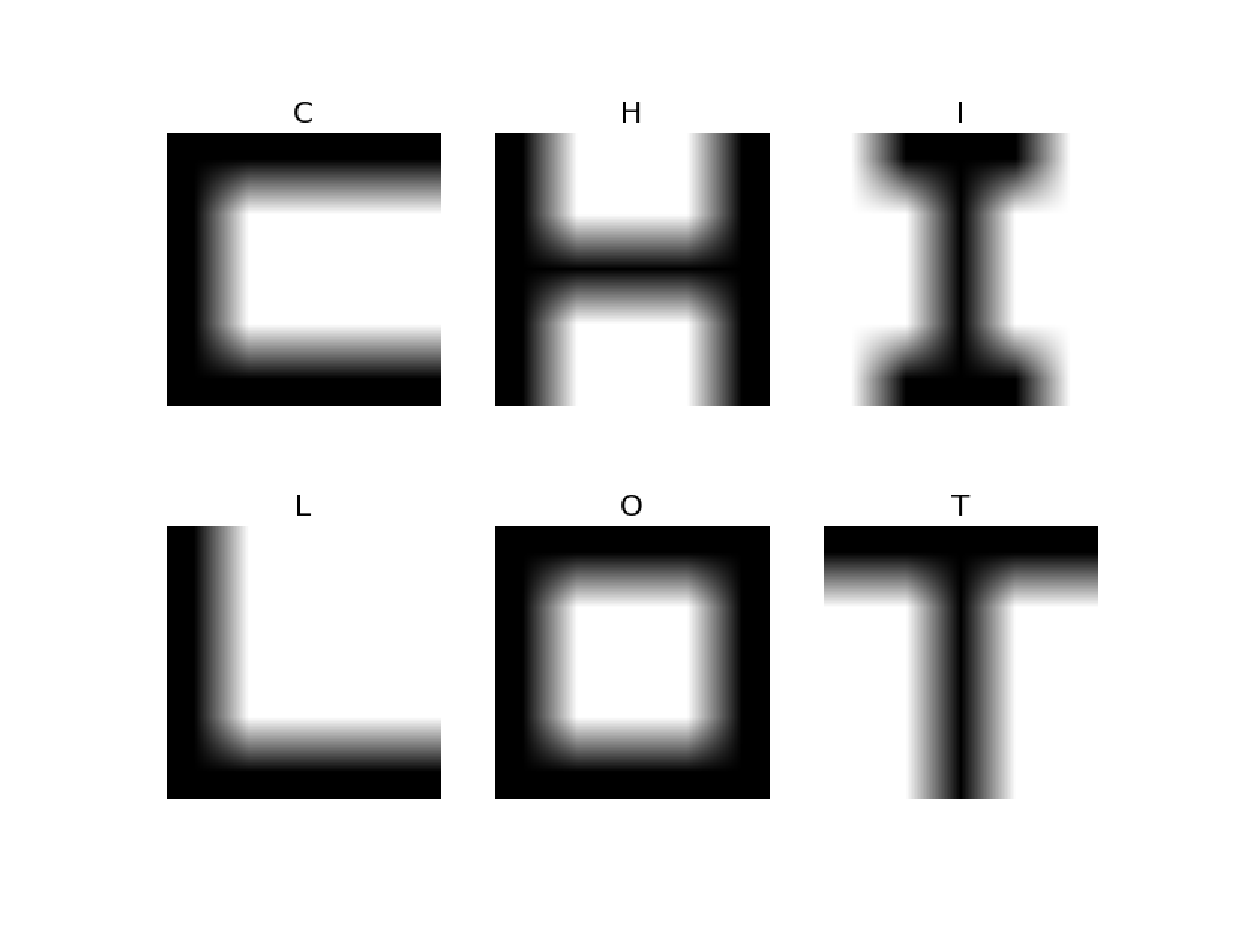
\includegraphics[width=\columnwidth]{figs/alphabet_images}
    \caption{利用画像}
  \label{fig:original-images}
\end{figure}
%%% -------------------------------------------------


%%% -------------------------------------------------
\section{2種類画像における識別性能}\label{sec:two-label-performance}
全6種の画像から2つを選択する組み合わせは15種類ある.
各組み合わせにおける識別性能は\figref{two-label-performance}
のようになり,組み合わせによる識別性能の変動は小さいと言える.
\begin{figure}[htpb]
  \centering
    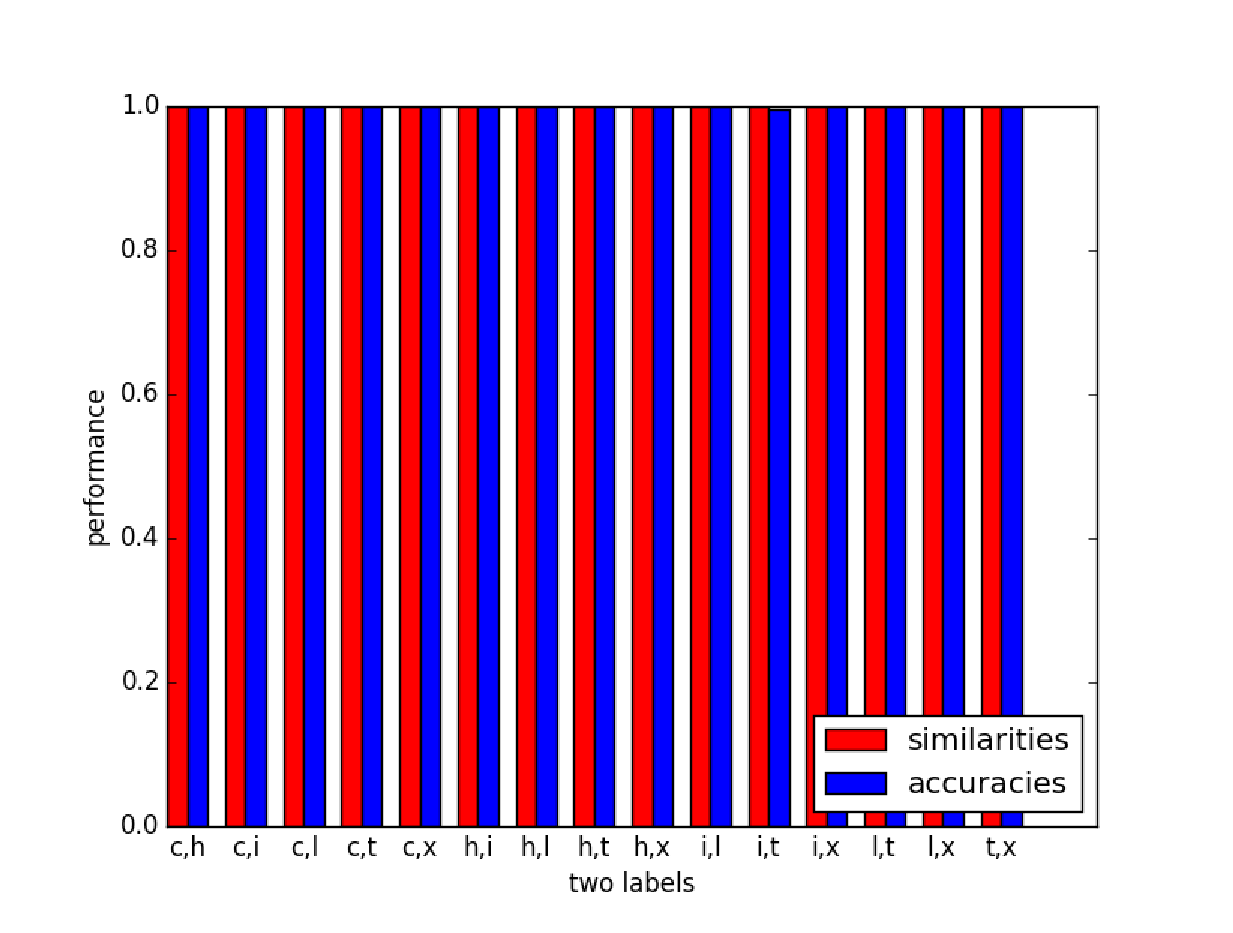
\includegraphics[width=\columnwidth]{figs/two_label_performance}
    \caption{2種類画像における識別性能}
    \label{fig:two-label-performance}
\end{figure}
%%% -------------------------------------------------


%%% -------------------------------------------------
\section{画像の種類数による想起性能変化}
画像の種類を2から6まで変化させ,想起性能の変化を調べた.
\ref{sec:two-label-performance}より,組み合わせによる性能の変動が小さいことから
画像種類の変化に対して全ての組み合わせを調べずに,
アルファベット順に各種類数分を選択し性能変化を見ることとする.

\figref{labels-performance}に示すように,画像の種類を増加させると想起性能は下がる.
しかし正答率(accuracy)は大きく減少する一方で,
類似度平均(similarity)はそれほど減少しないということがわかる.
\begin{figure}[htpb]
  \centering
    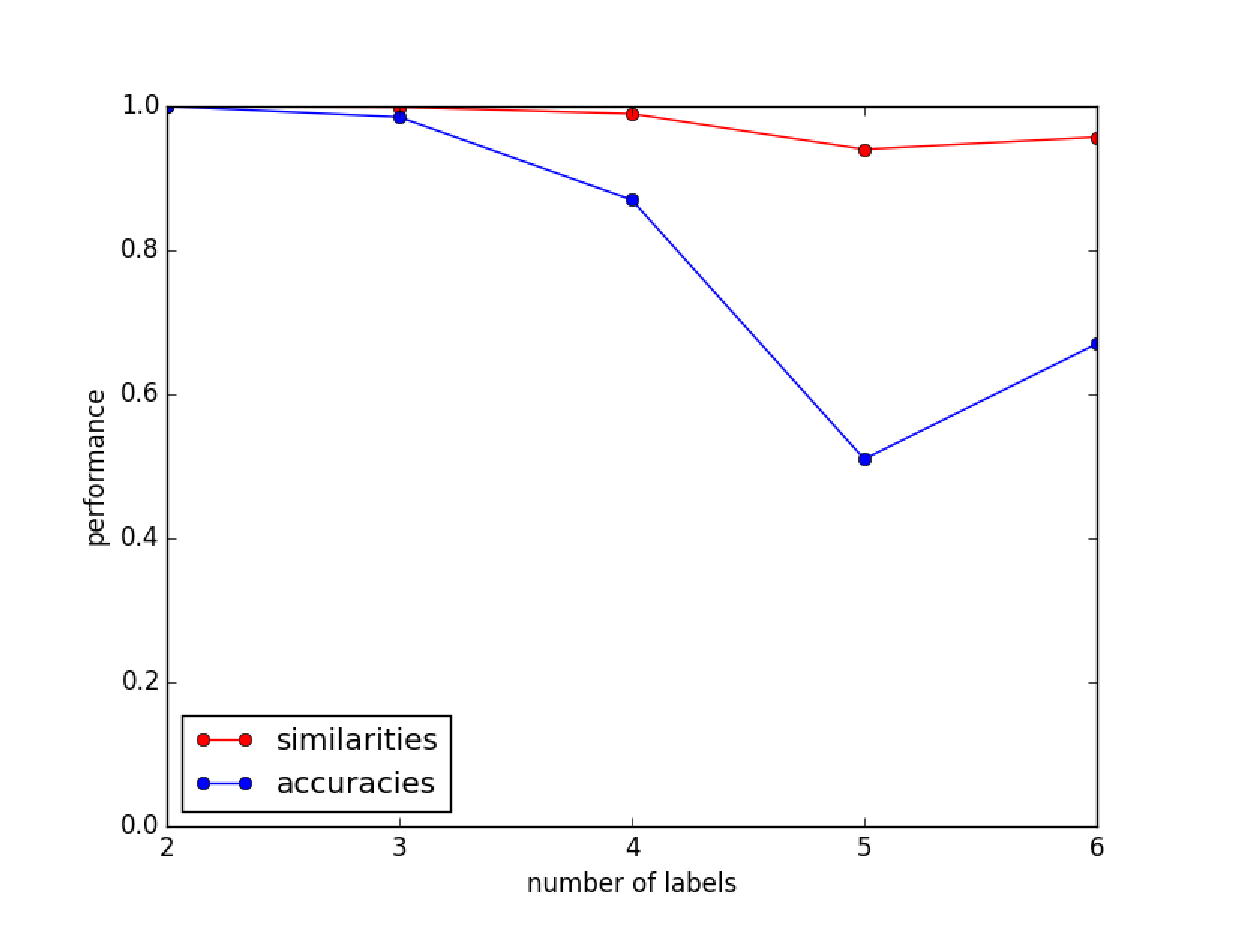
\includegraphics[width=\columnwidth]{figs/labels_performance}
    \caption{画像の種類数による想起性能変化}
    \label{fig:labels-performance}
\end{figure}
%%% -------------------------------------------------


%%% -------------------------------------------------
\section{入力画像のノイズ量による想起性能変化}
入力画像に加えるノイズ量を5から50\%まで変化させ,想起性能の変化を調べた.
%%% -------------------------------------------------


%%% Bibliography ------------------------------------
\begin{thebibliography}{9}
  \bibitem{bib1} Samuel R.Buss,"Introduction to Inverse Kinematics with Jacobian Transpose,Pseudoinverse and Damped Least Squares methods"
\end{thebibliography}
%%% -------------------------------------------------


\end{document}
